\documentclass[a4paper, 11pt]{article}
\usepackage{amsmath}
\usepackage{amssymb}
\usepackage[T1]{fontenc}
\usepackage[utf8x]{inputenc}
\usepackage{lmodern}
\usepackage{graphicx}
\graphicspath{ {./images/} }
\usepackage[english]{babel} 
\usepackage{natbib}
\usepackage{cite}
\usepackage[parfill]{parskip}
\usepackage{enumerate}
\usepackage{float}%for image positions
\usepackage{hyperref}
\hypersetup{
  colorlinks,
  citecolor=black,
  filecolor=black,
  linkcolor=black,
  urlcolor=black
}
\usepackage{amsthm}
\newtheorem{theorem}{Theorem}[section]
\newtheorem{lemma}[theorem]{Lemma}
\newtheorem{proposition}[theorem]{Proposition}
\newtheorem{axiom}[theorem]{Axiom}
\newtheorem{invariant}[theorem]{Invariant}
\newtheorem{breakpoint}[theorem]{Breakpoint}
\newtheorem{problem}{Problem}
\newtheorem{definition}{Definition} 
\usepackage{algorithm}
\usepackage{algpseudocode}
\usepackage{pifont}
\usepackage{multirow,array}
\usepackage{centernot}
\usepackage{listings}
\usepackage{xcolor}

\lstdefinestyle{base}{
  language=C,
  emptylines=1,
  breaklines=true,
  basicstyle=\ttfamily\color{black},
  moredelim=**[is][\color{red}]{@}{@},
}

\usepackage{comment} % enables the use of multi-line comments (\ifx \fi) 
\usepackage{lipsum} %This package just generates Lorem Ipsum filler text. 
\usepackage{fullpage} % changes the margin

\begin{document}
\noindent
\large\textbf{Assignment 1} \hfill \textbf{Kim Hammar} \\
\normalsize ID2204 \hfill  \textbf{Mallu} \\
Constraint Programming \hfill Due Date: 7 April 2017\\

\section*{Sudoku}
\subsection*{Constraints}
The sudoku model uses $9+9+9$ distinct constraints:

$\forall r \in \text{ rows }\quad distinct(r)$\\
$\forall c \in \text{ columns }\quad distinct(c)$\\
$\forall s \in \text{ 3x3-squares }\quad distinct(s)$

\subsection*{Branching and Propagation}
The solvability of this sudoku model depends a lot on the branching strategy and propagator strengths. For instance if we choose to go with a lower propagation constraint, which implies more search, the branching strategy is very essential. E.g when using \texttt{IPL\_VAL} as propagation level for all constraints, if we choose first-fail branching heuristic the model is solved rather quickly (< 1s, 214 nodes, 103 failures for sudoku instance 0), however if we choose the last-fail branching heuristic the model is not solved even solved after > 2min search. A very interesting note here is that if we choose a stronger propagation level, like \texttt{IPL\_DOM} the branch strategy is of less importance since some sudoku instances can even be solved without any search at all by using strong propagation, e.g no matter the branching strategy sudoku instance $0$ can be solved in the same time (< 1s, 1 node, 0 failures, 172 propagations) by using propagation level \texttt{IPL\_DOM}.

Illustration of the difference in amount of search necessary:

\begin{figure}[H]
  \begin{center}
    \scalebox{0.90}{
      
\includegraphics{dom1.pdf}
    }
    \caption{Search tree for propagation level \texttt{IPL\_DOM}}
    \label{fig:dom1}
  \end{center}
\end{figure}

\begin{figure}[H]
  \begin{center}
    \scalebox{0.90}{
      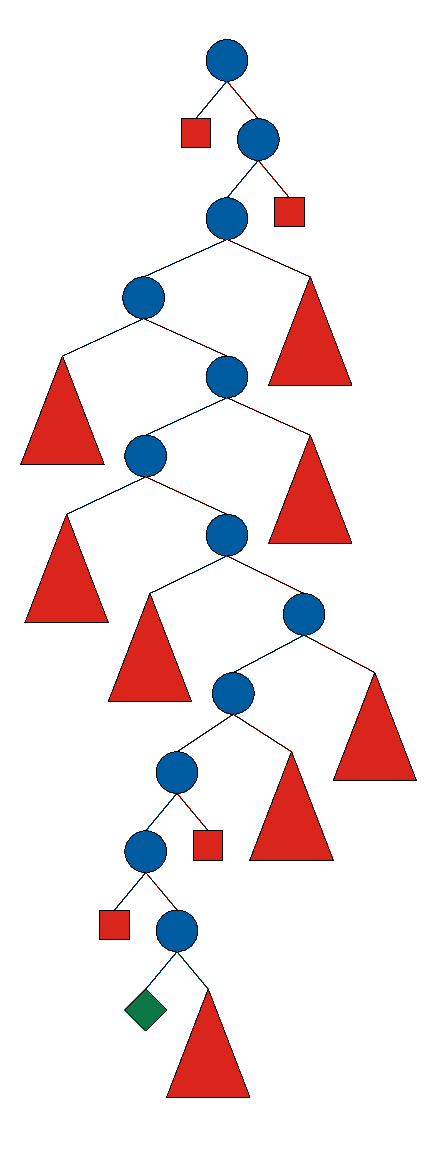
\includegraphics{val1_ff.pdf}
    }
    \caption{Search tree for propagation level \texttt{IPL\_VAL} and first-fail branch heuristic}
    \label{fig:val1_ff}
  \end{center}
\end{figure}

\texttt{IPL\_SPEED} and \texttt{IPL\_BASIC} propagation resulted in similar search tree as \texttt{IPL\_VAL}.

Bounds-consistency gave propagation somewhere inbetween \texttt{IPL\_DOM} and \texttt{IPL\_VAL} and solved sudoku instance $0$ in less than $1s$ with $23$ nodes and $10$ failures. With bounds-consistency it is also possible to solve sudoku instance $0$ with last-fail heuristic in less than $1s$ (39 nodes, 18 failures).

\begin{figure}[H]
  \begin{center}
    \scalebox{0.90}{
      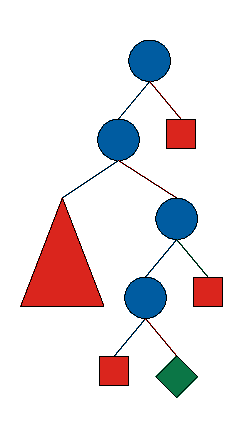
\includegraphics{bnd_ff.pdf}
    }
    \caption{Search tree for propagation level \texttt{IPL\_BND} and first-fail branch heuristic}
    \label{fig:bnd_ff}
  \end{center}
\end{figure}

To conclude, for this sudoku model stronger propagation is preferred, with \texttt{IPL\_DOM} it is possible to achieve backtrack-free search and a solution in polynomial time. 

\section*{n-Queens With 0/1 Variables}
Modelling the problem as a $n \times n$ matrix using $0/1$ variables means having one constraint per row, column, diagonal. 
\subsection*{Formulation as a CSP}
n-Queens, $n = 4$\\
$CSP = \langle \mathcal{V}, \mathcal{U}, \mathcal{C} \rangle$

Variables $\mathcal{V} = \{x_{1,1}, \ldots, x_{n,n}\}$ ($x_{col,row}$)

Universe $\mathcal{U} = \{0,1\}$

Constraints $\mathcal{C} = \{c_1,c_2,c_3,c_4,...c_{18}\}$\\
Constraints for columns: $\{c_1, \ldots, c_4\}$\\
Constraints for rows:$\{c_5, \ldots, c_9\}$\\
Constraints for diagonals:$\{c_{10}, \ldots, c_{18}\}$

Example constraint $c_1$ for column $1$:\\
var($c_1$) $= \langle x_{1,1}, x_{1,2}, x_{1,3}, x_{1,4} \rangle$\\
sol($c_1$) $= \{\langle 1,0,0,0 \rangle, \langle 0,1,0,0\rangle, \langle 0,0,1,0\rangle, \langle 0,0,0,1 \rangle\}$

Example constraint $c_5$ for row $1$:\\
var($c_5$) $= \langle x_{1,1}, x_{1,2}, x_{1,3}, x_{1,4} \rangle$\\
sol($c_5$) $= \{\langle 1,0,0,0 \rangle, \langle 0,1,0,0\rangle, \langle 0,0,1,0\rangle, \langle 0,0,0,1 \rangle\}$

Example constraint $c_{10}$ for diagonal $x_{1,4}-x_{4,1}$:\\
var($c_{10}$) $= \langle x_{1,4}, x_{2,3}, x_{3,2}, x_{4,1} \rangle$\\
sol($c_{10}$) $= \{\langle 1,0,0,0 \rangle, \langle 0,1,0,0\rangle, \langle 0,0,1,0\rangle, \langle 0,0,0,1 \rangle \langle 0,0,0,0 \rangle\}$

\subsection*{Model}
\subsubsection*{Variables}
\texttt{Matrix<IntVarArray>} of size $n \times n$
\subsubsection*{Constraints}
The constraints can be implemented in Gecode by asserting that the sum of the rows and columns should be $1$ (no two queens can share row/column) and that for each diagonal the sum can at most be $1$ (there can only be at most one queen in each diagonal).

$\forall c \in \text{ Matrix.columns } \quad c.sum() \equiv 1$\\
$\forall r \in \text{ Matrix.rows } \quad r.sum() \equiv 1$\\
$\forall d \in \text{ Matrix.diagonals } \quad d.sum() \leq 1$\\

\subsubsection*{Branching}
\textit{What can you do about branching?} Not that much as it seems (compared to other constraint problems). Since the variable domains are from the start very small $\{1,2\}$, the effect of switching between  for example \texttt{INT\_VAR\_SIZE\_MIN} and \texttt{INT\_VAR\_SIZE\_MAX} is not as evident compared to the queen-model with variable domains of larger size ($\{1, \ldots , 9 \}$).

After doing some experiments mainly with \texttt{INT\_VAR\_NONE}, \texttt{INT\_VAR\_SIZE\_MIN}, \texttt{INT\_VAR\_RND}, \texttt{INT\_VAL\_SIZE\_MAX}, \texttt{INT\_VAL\_SIZE\_MIN}. We have found that \texttt{INT\_VAR\_SIZE\_MIN} (first-fail heuristic) was the most successful, choosing the value ($0$ or $1$) heuristic was of minor importance regarding performance, but of course affected what type of solutions was found first.

The first-fail-heuristic outperformed \texttt{INT\_VAR\_RND} by a factor of $\sim 5$ and in fact \texttt{INT\_VAR\_NONE} and \texttt{INT\_VAR\_SIZE\_MIN} gave similar results, fail-first slightly better only.

$n = 5$, first-fail vs random heuristic search trees:

\begin{figure}[H]
  \begin{center}
    \scalebox{0.90}{
      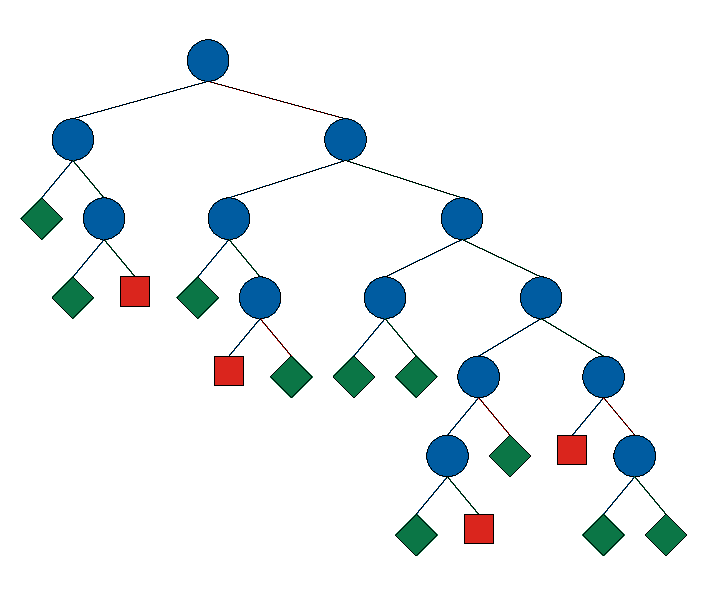
\includegraphics{first_fail_5_all.pdf}
    }
    \caption{First-fail heuristic finding all solutions for problem instance $n = 5$}
    \label{fig:ff5}
  \end{center}
\end{figure}

\begin{figure}[H]
  \begin{center}
    \scalebox{0.90}{
      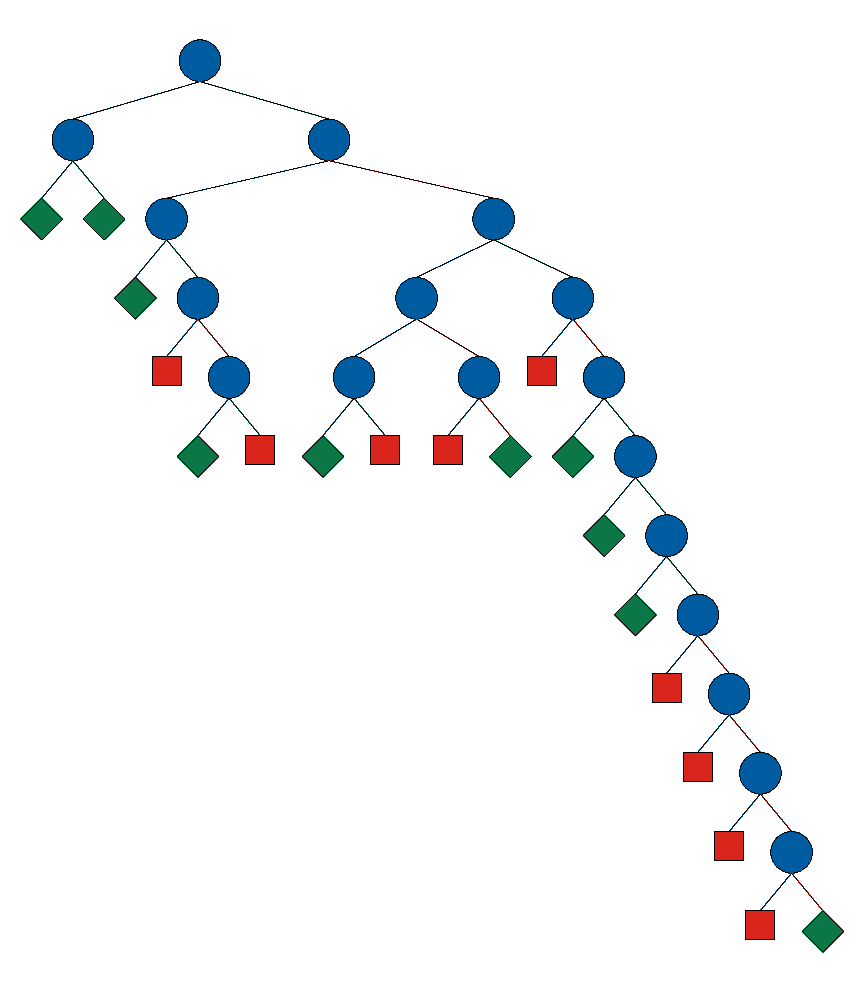
\includegraphics{rnd_all_5.pdf}
    }
    \caption{Random heuristic finding all solutions for problem instance $n = 5$}
    \label{fig:rnd5}
  \end{center}
\end{figure}
\subsection*{Pros and Cons}
\textbf{Pros}:
\begin{itemize}
\item Less constraints than for example using the binary-constraints model in the example. Since propagators are ran one at a time this is in theory good from a performance perspective. Also, in some cases since propagation is not compositional, fewer larger constraints can give better propagation.
\item Very small domains for each value: $\{0,1\}$ compared to the non-matrix approach with domains of $\{0, \ldots, n\}$, but this is a trade-off since the matrix-model contains a lot more variables ($n^2$ vs $n$) compared to the example.
\item Very intuitive model and probably the model chosen by someone familiar with the n-queens problem but not with constraint-programming techniques.
\end{itemize}
\textbf{Cons}:
\begin{itemize}
\item The matrix model is less memory-efficient.
\item A lot more variables.
\item The example enforces one constraint just by modelling in a smart way: one queen per column constraint is enforced by the one-dimensional array. This is not utilised in the matrix-model.
\end{itemize}
\section*{How to run}
Both Gecode models are subclasses of \texttt{Script} and you can run the from commandline with all options provided by default Gecode-script. For the sudoku model you can also specify which of the example-problems you want to solve by adding the flag: \texttt{-sudoku <num>}.

\textbf{Examples}:

Find all solutions to the 5-queens problem, not using GIST:
\begin{verbatim}
./queens -mode solution -solutions 0 10

.
.

Queens Board Solution: 
. . . . . . . . . Q 
. . . . . . . Q . . 
. . . . Q . . . . . 
. . Q . . . . . . . 
Q . . . . . . . . . 
. . . . . Q . . . . 
. Q . . . . . . . . 
. . . . . . . . Q . 
. . . . . . Q . . . 
. . . Q . . . . . . 
-------------------

Initial
        propagators: 58
        branchers:   1

Summary
        runtime:      0.088 (88.935 ms)
        solutions:    724
        propagations: 335188
        nodes:        11809
        failures:     5181
        restarts:     0
        no-goods:     0
        peak depth:   13
\end{verbatim}

Solve sudoku example number $0$ without gist and propagation-level: Domain-consistency:
\begin{verbatim}
./sudoku -sudoku 0 -mode solution -ipl dom

Sudoku
-------------------------
|3|7|8  |2|6|5|  |9|1|4|
|5|9|6  |8|1|4|  |7|3|2|
|1|4|2  |7|3|9|  |5|6|8|

|2|1|7  |3|8|6|  |4|5|9|
|8|5|4  |9|7|1|  |6|2|3|
|6|3|9  |5|4|2|  |8|7|1|

|7|8|5  |4|2|3|  |1|9|6|
|4|6|3  |1|9|7|  |2|8|5|
|9|2|1  |6|5|8|  |3|4|7|
-------------------------

Initial
        propagators: 27
        branchers:   1

Summary
        runtime:      0.000 (0.752 ms)
        solutions:    1
        propagations: 172
        nodes:        1
        failures:     0
        restarts:     0
        no-goods:     0
        peak depth:   0

\end{verbatim}
\bibliography{references}{}
\bibliographystyle{plain}
\end{document}